\documentclass[aspectratio=169]{beamer}
\usetheme{default}
\usecolortheme{dove}

\usepackage{graphicx}
\graphicspath{./Figures/}

\usepackage[
    natbib=true,
    backend=bibtex,
    style=authoryear,
    maxcitenames=1
    ]{biblatex}

\usepackage{pdflscape}
\usepackage[makeroom]{cancel}

\newcommand{\old}{\text{old}}
\newcommand{\new}{\text{new}}

\setbeamersize{text margin left=5mm,text margin right=5mm} 

\addbibresource{/home/georgy/Documents/Papers/bibliography.bib}

\title{Optimising Replay for Partially Observable Domains}
\subtitle{Georgy, lab meeting 09/03/22}
\date{}

\begin{document}

\begin{frame}
    \titlepage

    % \vspace{-2cm}

    % \begin{minipage}[]{\textwidth}
    %     \centering
    %     Cognitive Maps discussion group
    % \end{minipage}
\end{frame}

\begin{frame}
    \frametitle{talk outline}
    \begin{itemize}
        \item[$\circ$] planning
        \item[$\circ$] DYNA, prioritised sweeping
        \item[$\circ$] explore-exploit
        \item[$\circ$] normative theory of hippocampal replay
        \item[$\circ$] replay in Bayesian bandits
        \item[$\circ$] replay in BAMDPs
        \item[$\circ$] limitations and future directions
    \end{itemize}

    % \begin{minipage}[b!]{\textwidth}
    %     \raggedright
    %     {\footnotesize \citet{behrensWhatCognitiveMap2018}}
    % \end{minipage}
\end{frame}

\begin{frame}
    \frametitle{planning}
    \begin{itemize}
        \item[$\circ$] generally speaking, planning refers to the process of computing a policy -- i.e., coming up with an action to execute
        \item[$\circ$] in value-based planning, this is achieved by estimating values associated with the available actions 
        \item[$\circ$] planning typically requires a model of the environment 
        \item[$\circ$] several aproaches exist: dynamic programming (DP), sample/simulation-based
    \end{itemize}
\end{frame}

\begin{frame}
    \frametitle{planning $\rightarrow$ dynamic programming} 
    \begin{itemize}
        \item[$\circ$] Bellman optimality equation
        $$ V^*(s) = \max_a \sum_{s'}\mathcal{P}_{ss'}^a[\mathcal{R}_{ss'}^a + \gamma V^*(s')] $$ 
        \item[$\circ$] value iteration is one example value-based planning algorithm
        $$ V_k(s) \leftarrow \max_a \sum_{s'}\mathcal{P}_{ss'}^a[\mathcal{R}_{ss'}^a + \gamma V_{k-1}(s')] $$ 
        \item[$\circ$] assumes a known model of the environment $\mathcal{P}_{ss'}^a$ 
        \item[$\circ$] performs synchronous sweeps over all states; computationally expensive; time-consuming
    \end{itemize}
\end{frame}

\begin{frame}
    \frametitle{planning $\rightarrow$ MCTS} 
    \begin{minipage}{0.7\textwidth}
        \begin{figure}
            \centering
            \includegraphics[width=1\textwidth]{mcts.png}
        \end{figure}    
    \end{minipage}%
    \begin{minipage}{0.3\textwidth}
        \begin{itemize}
            \item[$\circ$] MCTS is a simulation-based planning algorithm
            \item[$\circ$] Tree and rollout policies
            \item[$\circ$] Difficult to balance exploration and exploitation
        \end{itemize}    
    \end{minipage}
\end{frame}

\begin{frame}
    \frametitle{DYNA} 
    \begin{figure}
        \centering
        \includegraphics[width=0.4\textwidth]{dyna.png}
    \end{figure}
    \hspace*{\fill} {\footnotesize \citet{suttonIntegratedArchitecturesLearning1990}}
    \begin{itemize}
        \item[$\circ$] DYNA is an integrated architecture
        \item[$\circ$] combines a \emph{reactive} MF policy and a \emph{deliberate} MB system 
        \item[$\circ$] MB system is used offline to provide additional training to MF values
    \end{itemize}
\end{frame}

\begin{frame}
    \frametitle{DYNA $\rightarrow$ example} 
    \begin{figure}
        \centering
        \includegraphics[width=0.7\textwidth]{dyna_eg.png}
    \end{figure}
    \begin{itemize}
        \item[$\circ$] agent discovers online prediction erros (e.g., a goal)
        \item[$\circ$] model inversion to additionally train MF values 
        $$ Q^{MF}(s,a) \leftarrow Q^{MF}(s,a) + \alpha [R^{MB}(s') + \gamma \max_{a'} Q^{MB}(s', a') - Q^{MF}(s,a)] $$
        \item[$\circ$] asynchronous DP
    \end{itemize}
\end{frame}

\begin{frame}
    \frametitle{prioritised sweeping} 
    \begin{itemize}
        \item[$\circ$] asynchronous DP updates can be optimised 
        \item[$\circ$] online discovery of a prediction error results in high offline prediction errors for the immediately preceeding states
        \item[$\circ$] the idea of prioritised sweeping \parencite{moorePrioritizedSweepingReinforcement1993} is to execute the individual updates according to a priority queue, for instance:
        $$ p(s, a) = | Q^{MF}(s,a) + \alpha [R(s') + \gamma \max_{a'} Q^{MF}(s', a') - Q^{MF}(s,a)] \,| $$
    \end{itemize}
\end{frame}

\begin{frame}
    \frametitle{prioritised sweeping $\rightarrow$ example} 
\end{frame}

\begin{frame}
    \frametitle{explore-exploit} 
    \begin{itemize}
        \item[$\circ$] Optimal behaviour necessitates optimal balance of exploration and exploitation
        \item[$\circ$] Multiple heuristics have been devised to encourage exploration
        \item[$\circ$] One prominent heuristic is called an \emph{exploration bonus} 
        \item[$\circ$] \citet{suttonDynaIntegratedArchitecture1991} proposed to add an exploration bonus to the values of state-action pairs which have not been visited recently:
        $$ Q^{MB}(s,a) \leftarrow Q^{MB}(s,a) + \kappa \sqrt{\epsilon_{(s,a)}} $$
        where $\epsilon_{(s,a)}$ grows with the number of time steps elapsed since the state-action pair $(s,a)$ was last tried, and 
        $\kappa$ controls the rate of exploration
    \end{itemize}
\end{frame}

\begin{frame}
    \frametitle{explore-exploit $\rightarrow$ DYNA-Q+} 
    \begin{minipage}{0.6\textwidth}
        \begin{figure}
            \centering
            \includegraphics[width=0.85\textwidth]{dynaqplus.png}
        \end{figure}
    \end{minipage}%
    \begin{minipage}{0.4\textwidth}
        \begin{itemize}
            \item[$\circ$] note that this exploration bonus is myopic
            \item[$\circ$] propagates from distal locations due to the $Q$-learning rule 
            \item[$\circ$] however, it is blind towards what could be the consequences of exploration 
        \end{itemize}
    \end{minipage}
\end{frame}

\begin{frame}
    \frametitle{hippocampal replay}
    \begin{figure}
        \centering
        \includegraphics[width=0.65\textwidth]{replay_eg.jpg}
    \end{figure}
    \hspace*{\fill} {\footnotesize \citet{drieuHippocampalSequencesExploration2019}} 
    \begin{itemize}
        \item[$\circ$] reinstatement of behaviourally-relevant neural activity during periods of quiet wakefullness and sleep (offline periods)
        \item[$\circ$] the order of the replayed experiences is highly specific
        \item[$\circ$] can proceed in forward and reverse directions
        \item[$\circ$] forward replay seems to be predictive of the subsequent animal choices; 
        reverse replay is highly sensitive to reward
    \end{itemize}
\end{frame}

\begin{frame}
    \frametitle{hippocampal replay $\rightarrow$ normative theory}

    \begin{itemize}
        \item[$\circ$] Mattar \& Daw (2018) realised that hippocampal replay might be a candidate mechanism for offline generative planning -- 
        acting in accordance with the DYNA system by supplying MB information to the animal's MF policy
        \item[$\circ$] each replay experience, according to Mattar \& Daw, corresponds to an update of an MF value for a state-action pair 
        \item[$\circ$] each replay update therefore changes the animal's policy at the state where that update is executed
        \item[$\circ$] the fact that the order in which replay experiences proceed is highly specific suggests some sort of prioritisation (prioritised sweeping) 
    \end{itemize}
\end{frame}

\begin{frame}
    \frametitle{hippocampal replay $\rightarrow$ normative theory}
    \begin{itemize}
        \item[$\circ$] by the repeated unrolling of $v_{\pi_\new}(s) - v_{\pi_\old}(s)$, where $s$ is the animal's current location, M\&D showed that 
        the value of computation (i.e., replay update) performed at state $s_k$ for action $a_k$ can be decomposed into two terms
        $$ \text{EVB}(s_k, a_k) = \sum_{s'\in \mathcal{S}} \underbrace{\sum_{i=0}^{\infty} \gamma^i P(s \rightarrow s', i, \pi_{\old})}_{\text{Need}} \times \underbrace{\sum_a [\pi_{\new}(a\mid s') - \pi_\old (a\mid s')]q_{\pi_\new}(s',a)}_{\text{Gain}} $$
        \item[$\circ$] Need is the expected discounted future occupancy of state $s'$ under the animal's policy prior to the update, $\pi_\old$
        \item[$\circ$] Gain quantifies the local policy improvement at the state where the potential replay update is considered  
    \end{itemize}
\end{frame}

\begin{frame}
    \frametitle{hippocampal replay $\rightarrow$ normative theory}
    \begin{figure}
        \centering
        \includegraphics[width=1\textwidth]{gain_need.png}
    \end{figure}
\end{frame}

\begin{frame}
    \frametitle{hippocampal replay $\rightarrow$ normative theory}
    $$ \text{EVB}(s_k, a_k) = \cancel{\color{red} \sum_{s'\in \mathcal{S}}} \underbrace{\sum_{i=0}^{\infty} \gamma^i P(s \rightarrow s', i, \pi_{\old})}_{\text{Need}} \times \underbrace{\sum_a [\pi_{\new}(a\mid s') - \pi_\old (a\mid s')]q_{\pi_\new}(s',a)}_{\text{Gain}} $$
    Assumptions of the M\&D model:
    \begin{itemize}
        \item[$\circ$] policy updates are local, and thus M\&D get rid of the first sum over $\mathcal{S}$
        \item[$\circ$] \begin{itemize}
            \item[$-$] Note this means that the benefit of policy change at a distal state is only considered at the animal's current state
        \end{itemize}
        \item[$\circ$] Gain is expressed in terms of the \emph{true} $Q$-values implied by the new policy, $q_{\pi_\new}$
        \item[$\circ$] the transition model $P$ is known   
    \end{itemize}
\end{frame}

\begin{frame}
    \frametitle{hippocampal replay $\rightarrow$ exploration?}
    \begin{figure}
        \centering
        \includegraphics[width=0.85\textwidth]{md_explore.png}
    \end{figure}
\end{frame}

\begin{frame}
    \frametitle{hippocampal replay $\rightarrow$ exploration?}
    \begin{itemize}
        \item[$\circ$] turns out the model of M\&D doesn't explore well
        \item[$\circ$] weird because the original intention of DYNA was to encourage exploration 
        \item[$\circ$] Need acts as a regulariser -- once a policy is learnt it biases the selection of 
        replay updates towards those states which the current policy already expects to visit (pure exploitation!)
        \item[$\circ$] Gain (in fact, Need as well) doesn't account for the potential information which can be learnt and utilised in the future 
    \end{itemize}
\end{frame}

\begin{frame}
    \frametitle{hippocampal replay $\rightarrow$ exploration?}
    \begin{minipage}[t]{0.5\textwidth}
        \begin{figure}
            \centering
            \includegraphics[width=0.9\textwidth]{replay_shortcut.png}
        \end{figure}
    \end{minipage}%
    \begin{minipage}[t]{0.5\textwidth}
        \begin{figure}
            \centering
            \includegraphics[width=1\textwidth]{replay_preplay.png}
        \end{figure}
    \end{minipage}
    \bigbreak
    \begin{tabular}{p{0.5\textwidth}p{0.5\textwidth}}
        \centering \citet{guptaHippocampalReplayNot2010} & \centering \citet{olafsdottirHippocampalPlaceCells2015}
    \end{tabular}
\end{frame}

\begin{frame}
    \frametitle{explore-exploit revisited}
    \begin{itemize}
        \item[$\circ$] in Bayesian RL, one often assumes some prior belief $b$ over the unknown parameters
        \item[$\circ$] in Bayes-adaptive MDPs [BAMDPs; \citet{duffQLearningBanditProblems1995}], the prior is 
        over the unknown transition model parameters: 
        $$ P(s'\mid s, a) = \int_{\Theta} P(s' \mid s, a, \theta) b(\theta) d\theta $$ 
        \item[$\circ$] once integrated out, the model becomes known; moreover, it incorporates the agent's epistemic uncertainty -- i.e., the 'known unknowns'
        \item[$\circ$] the resulting policies are known as Bayes-adaptive policies, since they optimally trade-off exploration and exploitation
    \end{itemize}
\end{frame}

\begin{landscape}
    \begin{frame}
        % \frametitle{planning in bandits}
        \begin{itemize}
            \item[$\circ$] planning in bandits can be visualised as belief trees
        \end{itemize}
        \begin{figure}
            \includegraphics[width=0.62\textwidth]{guez_bandits.png}
        \end{figure}
        \hspace*{\fill} {\footnotesize \citet{guezSampleBasedSearchMethods2015}}
        \begin{itemize}
            \item[$\circ$] optimal solution is known as the Gittins indices \parencite{gittinsBanditProcessesDynamic1979}, 
            which correspond to the DP solution in the belief space 
        \end{itemize}
    \end{frame}
\end{landscape}

\begin{frame}
    \frametitle{replay in Bayesian bandits}
    \begin{itemize}
        \item[$\circ$] we can do the same decomposition as in M\&D but for belief states:
        $$ \text{EVB}(b_k, a_k) = \gamma^h P(b_\rho \rightarrow b_k, h, \pi_\old) \times \sum_a [\pi_\new (a\mid b_k) - \pi_\old (a\mid b_k)]q_{\pi_\new}(a, b_k) $$ 
        \item[$\circ$] where $b_\rho$ is the prior belief at the root, and $h$ is the horizon of belief $b_k$
        \item[$\circ$] note that Need here is not cumulative; this is because each belief state can be visited at most once due to continual learning
    \end{itemize}
\end{frame}

\begin{landscape}
    \begin{frame}
        \begin{itemize}
            \item[$\circ$] each rectangle is a belief state 
            \item[$\circ$] colour intensity corresponds to Need, $\gamma^h P(b_\rho \rightarrow b_k, h, \pi_\old)$
            \item[$\circ$] each arrow is an action
            \item[$\circ$] blue numbers are $Q$-values 
            \item[$\circ$] in this tree example, the root belief is $(\alpha_0=5, \beta_0=1, \alpha_1=2, \beta_1=4)$
            \item[$\circ$] the tree policy is a softmax with $\beta=4$ 
        \end{itemize}
        \begin{figure}
            \includegraphics[width=0.45\textwidth]{trees/1/tex_tree_0.pdf}
        \end{figure}
    \end{frame}
\end{landscape}

\begin{landscape}
    \begin{frame}
        \begin{figure}
            \includegraphics[width=0.55\textwidth]{trees/1/tex_tree_0.pdf}
        \end{figure}
    \end{frame}
\end{landscape}

\begin{landscape}
    \begin{frame}
        \begin{figure}
            \includegraphics[width=0.55\textwidth]{trees/1/tex_tree_1.pdf}
        \end{figure}
    \end{frame}
\end{landscape}

\begin{landscape}
    \begin{frame}
        \begin{figure}
            \includegraphics[width=0.55\textwidth]{trees/1/tex_tree_2.pdf}
        \end{figure}
    \end{frame}
\end{landscape}

\begin{landscape}
    \begin{frame}
        \begin{figure}
            \includegraphics[width=0.55\textwidth]{trees/1/tex_tree_3.pdf}
        \end{figure}
    \end{frame}
\end{landscape}

\begin{landscape}
    \begin{frame}
        \begin{figure}
            \includegraphics[width=0.55\textwidth]{trees/1/tex_tree_4.pdf}
        \end{figure}
    \end{frame}
\end{landscape}

\begin{landscape}
    \begin{frame}
        \begin{figure}
            \includegraphics[width=0.55\textwidth]{trees/1/tex_tree_5.pdf}
        \end{figure}
    \end{frame}
\end{landscape}

\begin{landscape}
    \begin{frame}
        \begin{figure}
            \includegraphics[width=0.55\textwidth]{trees/1/tex_tree_6.pdf}
        \end{figure}
    \end{frame}
\end{landscape}

\begin{landscape}
    \begin{frame}
        \begin{figure}
            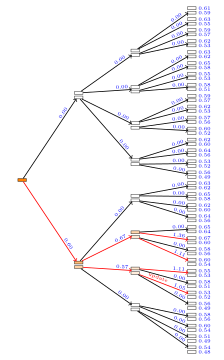
\includegraphics[width=0.55\textwidth]{trees/1/tex_tree_7.pdf}
        \end{figure}
    \end{frame}
\end{landscape}

\begin{landscape}
    \begin{frame}
        \begin{figure}
            \includegraphics[width=0.55\textwidth]{trees/1/tex_tree_8.pdf}
        \end{figure}
    \end{frame}
\end{landscape}

\begin{landscape}
    \begin{frame}
        \begin{figure}
            \includegraphics[width=0.55\textwidth]{trees/1/tex_tree_9.pdf}
        \end{figure}
    \end{frame}
\end{landscape}

\begin{landscape}
    \begin{frame}
        \begin{figure}
            \includegraphics[width=0.55\textwidth]{trees/1/tex_tree_10.pdf}
        \end{figure}
    \end{frame}
\end{landscape}

\begin{frame}
    \frametitle{replay in Bayesian bandits}
    \begin{itemize}
        \item[$\circ$] the effects of each consequitive update on the root value, $V(b_\rho)$, as well 
        as the value of the new (updated) policy evaluated in the tree, $V^\pi$   
    \end{itemize}
    \begin{figure}
        \centering
        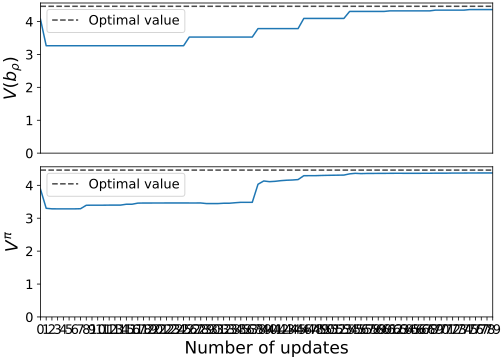
\includegraphics[width=0.55\textwidth]{trees/1/root_values.png}
    \end{figure}
\end{frame}

\begin{landscape}
    \begin{frame}
        \begin{figure}
            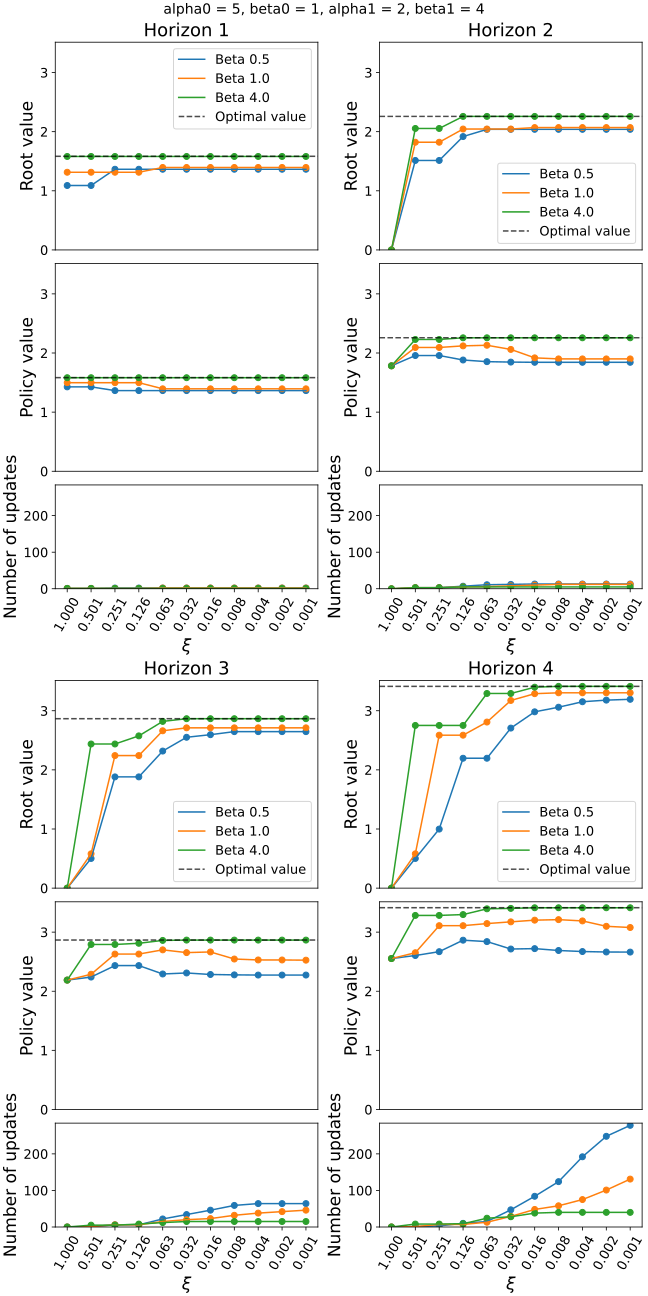
\includegraphics[width=0.48\textwidth]{trees/1/alpha05_beta01_alpha12_beta14_complete.png}
        \end{figure}
    \end{frame}
\end{landscape}

\begin{frame}
    \frametitle{replay in Bayesian bandits}
    \begin{itemize}
        \item[$\circ$] one more example
        \item[$\circ$] this time for the prior $(\alpha_0=14, \beta_0=10, \alpha_1=4, \beta_1=3)$ 
    \end{itemize}
\end{frame}

\begin{landscape}
    \begin{frame}
        \begin{figure}
            \includegraphics[width=0.55\textwidth]{trees/2/tex_tree_0.pdf}
        \end{figure}
    \end{frame}
\end{landscape}

\begin{landscape}
    \begin{frame}
        \begin{figure}
            \includegraphics[width=0.55\textwidth]{trees/2/tex_tree_1.pdf}
        \end{figure}
    \end{frame}
\end{landscape}

\begin{landscape}
    \begin{frame}
        \begin{figure}
            \includegraphics[width=0.55\textwidth]{trees/2/tex_tree_2.pdf}
        \end{figure}
    \end{frame}
\end{landscape}

\begin{landscape}
    \begin{frame}
        \begin{figure}
            \includegraphics[width=0.55\textwidth]{trees/2/tex_tree_28.pdf}
        \end{figure}
    \end{frame}
\end{landscape}

\begin{landscape}
    \begin{frame}
        \begin{figure}
            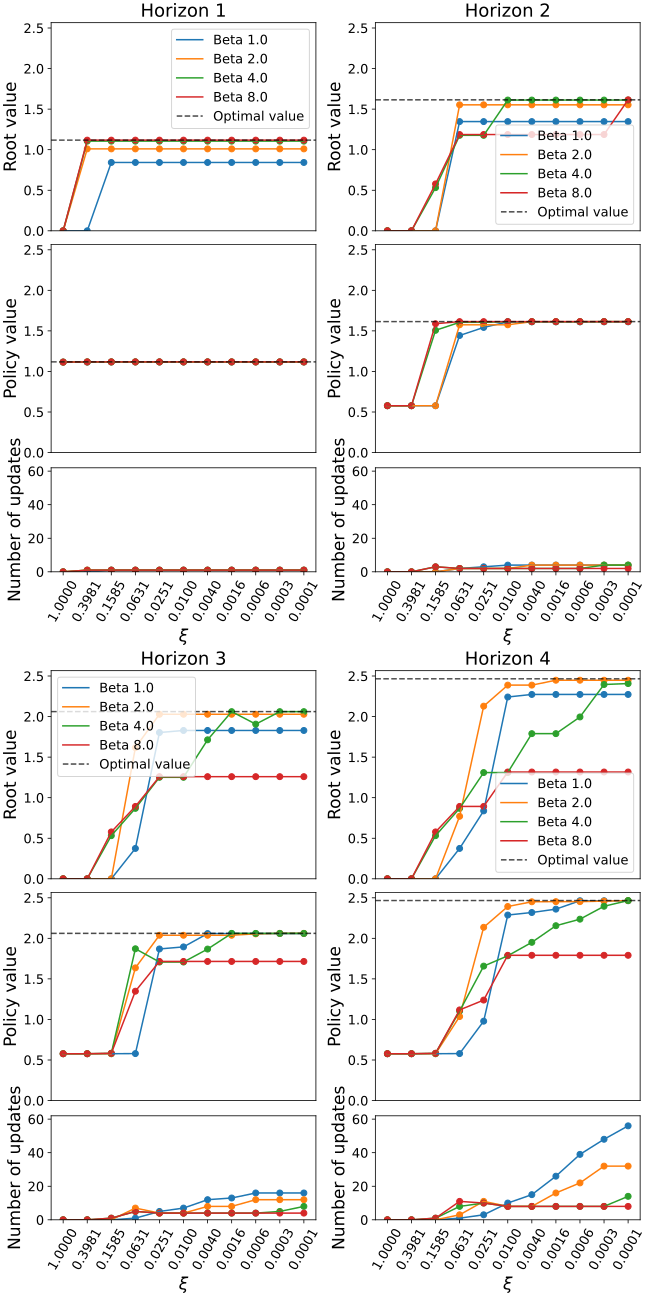
\includegraphics[width=0.48\textwidth]{trees/2/alpha014_beta010_alpha14_beta13_complete.png}
        \end{figure}
    \end{frame}
\end{landscape}

\begin{frame}
    \frametitle{replay in Bayesian bandits}
    \begin{itemize}
        \item[$\circ$] planning in belief space can be optimised
        \item[$\circ$] free generalisation for subsequent beliefs 
        \item[$\circ$] note the use of a softmax policy
        \item[$\circ$] we are ultimately interested in exploration in DYNA-like systems which have an MF policy; MB system needs to convince the MF policy that something is worth exploring
        \item[$\circ$] otherwise, the Need term $\gamma^h P(b_\rho \rightarrow b_k, h, \pi_\old)$ would be zero for those beliefs which the current MF policy doesn't expect to visit
        \item[$\circ$] similar issues in MCTS -- e.g., UCB  
    \end{itemize}
\end{frame}

\begin{frame}
    \frametitle{replay in BAMPDs}
    \begin{itemize}
        \item[$\circ$] in BAMDPs, we transition through belief states as well as physical states. Jointly, these are referred to as information states $z=\langle s, b\rangle$
        \item[$\circ$] the prioritisation in BAMDPs thus takes the following form:
        $$\text{EVB}(z_k, a_k) = \sum_{z'\in \mathcal{Z}}\sum_{i=0}^{\infty}\gamma^iP(z\rightarrow z', i, \pi_\old)\times \sum_a[\pi_\new(a\mid z') - \pi_\old(a\mid z')]q_{\pi_\new}(z', a)$$  
        \item[$\circ$] note that each $z=\langle s, b\rangle$ can still be visited at most once
        \item[$\circ$] we know, however, that although the belief changes continuosly, the agent should still expect to visit the same physical state over and over again
        \item[$\circ$] moreover, the summation over $\mathcal{Z}$ allows us to account for generalisation -- that is, how updates at single information states (revealing a piece of information) affect policy at other beliefs (not quite there yet)
    \end{itemize}
\end{frame}

\end{document}